
\section{Results}
Our primary database is used to reconstruct American Sign Language. 
The database is composed simply of two contiunous
runs of the signs of the letters for the complete 
alphabet, signed by the same actor. We test our method
on various sequences that include words in sign language, most of
which are not included in the database.

For our sparse marker set, we choose to use six markers as our
baseline in order to compare our technique to existing solutions. 
Using the method described in Section 5 to determine 
marker importance, the markers chosen are all of the fingertips
and one on the lower part of the index finger. We also choose a
marker set of three. The markers chosen are the fingertips of the 
middle, ring, and pinky fingers.

Sequences to be recontructed are initially recorded with a full
marker set. Markers not selected for the sparse marker set
are left out of the regression process.

Our method uses regression to predict principle components for
a sequence of motion. In Figure ~\ref{fig:BabySigns_comps}, we compare
the top three predicted components of a sequence of baby sign language
to the components of the original sequence with a full marker set. The
predicted components of six markers and three markers are shown.
Though there are differences, the motion of each component closely
follows that of the ground truth for both marker sets. This can be seen clearly
witha another reconstruced sequence in the video.

We also compare a regression mapping marker positions to principle components to
a regression mapping marker positions directly to joint angles. Figure
~\ref{fig:PCA_noPCA} shows that the average joint angle error for mapping
direclty to joint angles produces a much higher average joint angle error.
The reconstructed hand with six markers fails to reach every distinct pose
in the original animation.

We compare our marker set of six to the markers sets derived from the Manual
Selection Method presented by Hoyet et al. (2011) and the Cluster Pose Error
Method presented by Kang et al.(2012). Using the regression
method, our marker set produces a smaller average joint angle error per frame 
for all of our current sign language tests. The Manual Selection Method's
marker set consistently has the largest joint angle error. Figure
~\ref{fig:3_methods} shows these differences, again using the clip
of baby sign language as an example. The three distinct poses reached
in the baby sign language clip are also shown using the different marker
sets in Figure ~\ref{fig:BabySigns_methods}. Our marker set is consistently
close to the original pose where as
the two other marker fail at achieving at least one pose.\\

\begin{figure}[ht]
  \centering
  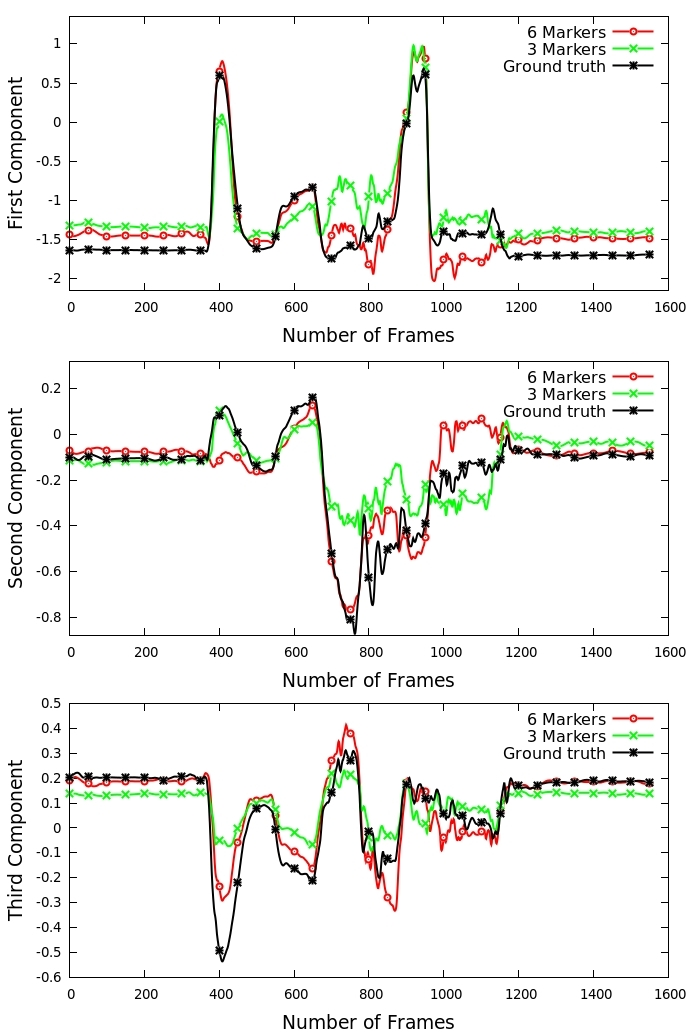
\includegraphics[trim = 28mm 0mm 0mm 0mm,
width=0.45\textwidth]{images/Components_babySigns1.jpg} %width=2.5in
  \caption{Comparison of the components of a reconstructed clip of baby
sign language when using 6 markers and 3 markers. Ground Truth is
the original clip recorded with 13 markers.}
  \label{fig:BabySigns_comps}
\end{figure}

\begin{figure}[ht]
  \centering
  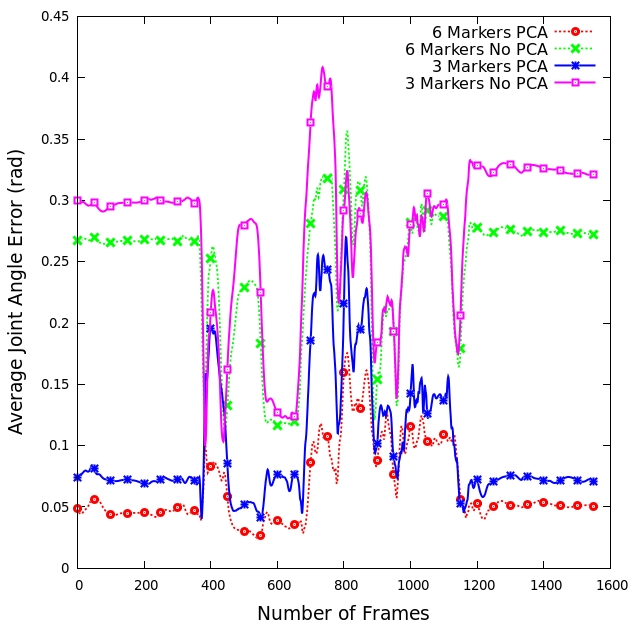
\includegraphics[trim = 28mm 0mm 0mm 0mm,
width=0.45\textwidth]{images/avgError_6_3_jangles_babySigns1.jpg} %width=2.5in
  \caption{Comparison of two regression methods: regression to principle
components and regression to joint angles.}
  \label{fig:PCA_noPCA}
\end{figure}

\begin{figure}[ht]
  \centering
  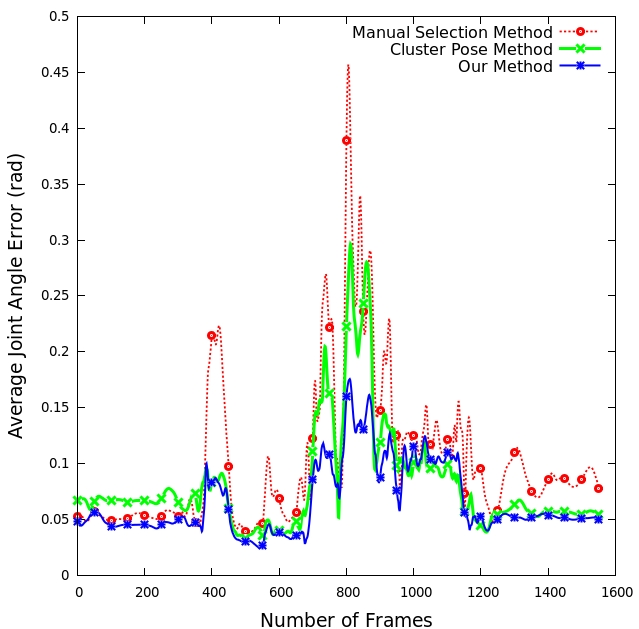
\includegraphics[trim = 28mm 0mm 0mm 0mm,
width=0.45\textwidth]{images/avgError_Marker_sets.jpg} %width=2.5in
  \caption{Comparison of three marker set selection methods that use 6 markers.}
  \label{fig:3_methods}
\end{figure}


\begin{figure}[ht]
  \centering
  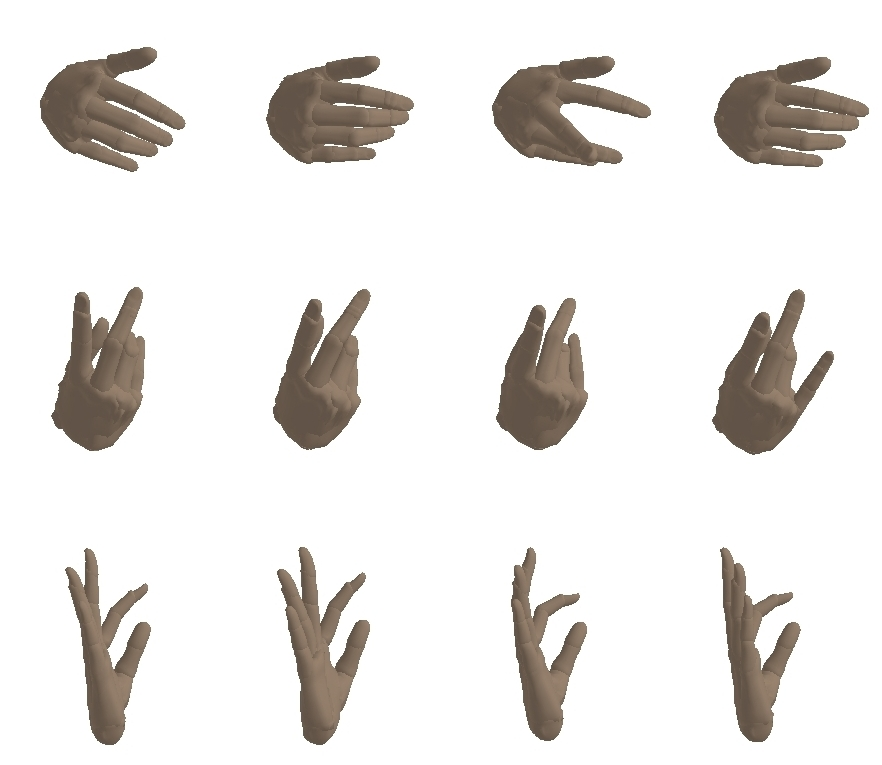
\includegraphics[trim = 28mm 0mm 0mm 0mm,
width=0.45\textwidth]{images/compiled_babySigns1_poses.jpg} %width=2.5in
  \caption{The three distinct poses of the baby sign language clip
reconstructed with the three different marker sets. They are compared to
the original poses.}
  \label{fig:BabySigns_methods}
\end{figure}





